%			
			\subsection{Dielectric Displacement Current}\label{sec:displacementcurrent}
%
				\begin{wrapfigure}{r}{0.47\textwidth}
					\centering%
					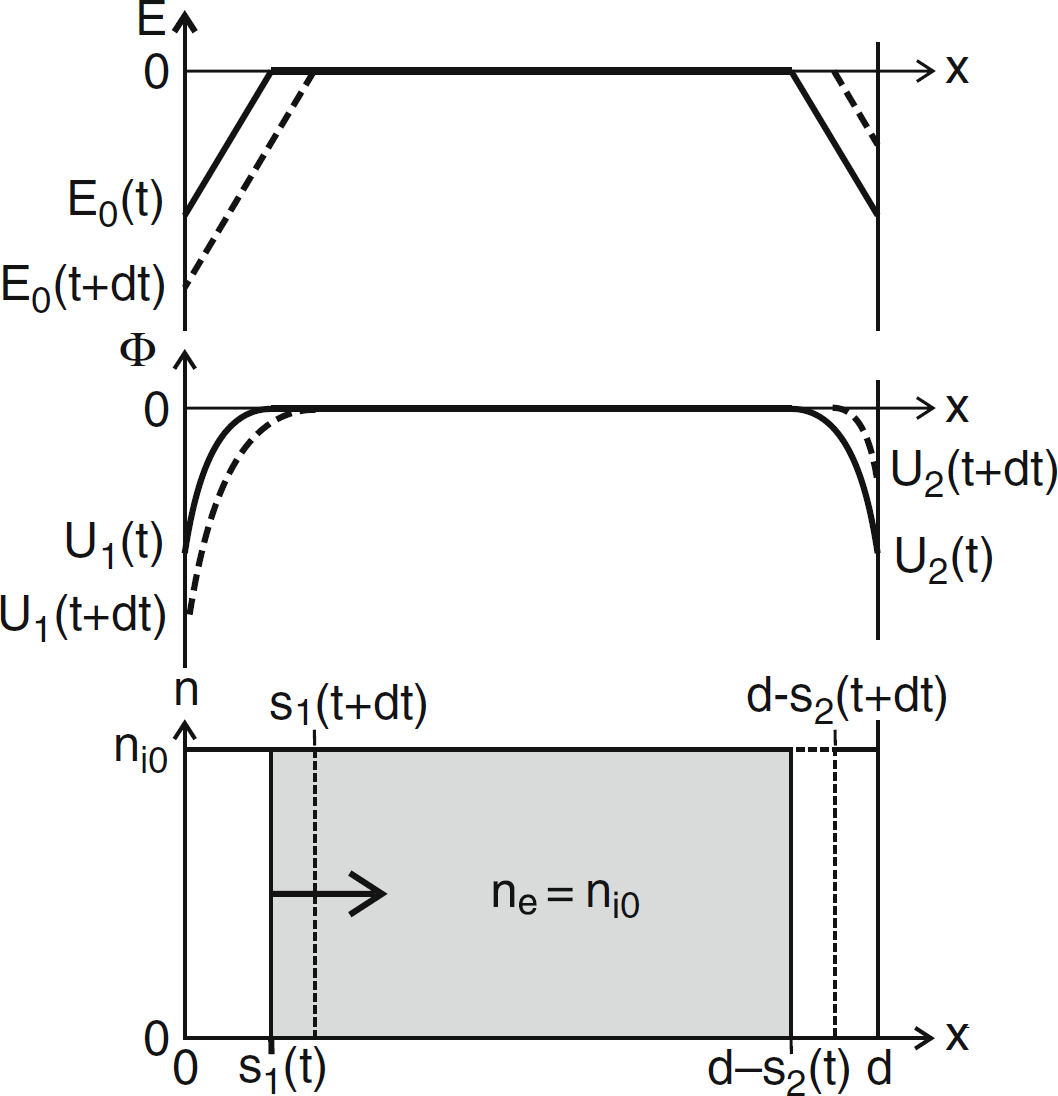
\includegraphics[width=0.45\textwidth]{figures/displacement_current_piel.png}%
					\caption{%
					One dimensional density, potential and electric field for an asymmetric, harmonically driven discharge. Note the moving sheaths border.~\cite{Piel10}}\label{fig:displacementcurrent}
				\end{wrapfigure}
%
				Due to their higher mobility and plasma frequency $\omega\ix{p,e}$, the electron distribution can follow an external excitation with a similarly high frequency much better than the heavier ions species. Because of that, one will assume those as nearly stationary, e.g.\@ $\omega\ix{p,i}\ll\omega\ix{p,e},\,\omega\ix{rf}\,$. Investigating the circumstances and consequences of this relation yields the displacement current $j\ix{d}$. \\
				Lets suppose there is an area of thickness $d$ in front of a negatively charged wall, where the electron ensity is negligible and the corresponding ion property constant at $n\ix{0,i}$. Thus an electric field of
%   	 
				\begin{align}
					E\ix{0}=-en\ix{0,i}d/\varepsilon\ix{0}
				\end{align}
%
				establishes. If the wall potential now decreases due to electron bombardment or external manipulation, the sheaths border moves further inside into the discharges volume with the velocity $u\ix{s}=\diff s\ix{1}/\diff t$. Thus, the sheath expansion and hence charge movement creates an additional \emph{displacement current} $j\ix{d}$, which is compensated with $j\ix{d,e}$ the electron current from this border displacement. Hence charge conservation and continuity is satisfied~\cite{Godyak90a}.
%
				\begin{align}
					j\ix{d}=-en\ix{0,i}u\ix{s}=-j\ix{d,e}
				\end{align}
%
				Electrons that are pushed out of this positive space-charge area then contribute to the plasma bulk density, and conclusively, to the quasi neutrality $n\ix{e}=n\ix{0,i}\,$. But in case of a harmonically driven discharge, the sheath in front of the opposing electrode is shrinking with $\diff s\ix{1}=-\diff s\ix{2}\,$. Hence, the bulks spatial expansion and position are oscillating sinusoidal, or: the sheaths thickness oscillates harmonically around a mean value, e.g\@ $s\ix{0}$. The associated voltage drop across the discharge~\cite{Piel10} between the sheath potentials $U\ix{1/2}$ would be
%
				\begin{align}
					\Delta U=U\ix{1}-U\ix{2}=-\frac{2en\ix{i,0}s\ix{0}}%
						{\varepsilon\ix{0}}\exp\left(\imag\omega t\right)
				\end{align}
%
